\chapter{Gestión y Planificación del proyecto}


\section{Metodología}

En el pasado, el desarrollo de software seguía un enfoque ad hoc (software a medida) y poco estructurado, lo que llevaba a problemas como retrasos, presupuestos desbordados, productos finales que no cumplían con las expectativas o proyectos inmanejables y difíciles de mantener. Era frecuente por tanto proyectos fallidos o de mala calidad. Como resultado, surgió la necesidad de establecer un marco de trabajo más formal y disciplinado para el desarrollo de software. Las metodologías de desarrollo proporcionan pues, un marco de trabajo y un conjunto de métodos que guían a los equipos de desarrollo a lo largo del ciclo de vida del proyecto. Es por tanto, a día de hoy, fundamental elegir una metodología que se adapte bien al proyecto.
Por lo general, las metodologías de desarrollo se clasifican en dos grandes grupos, tradicionales y ágiles. Se resume en la Tabla \ref{tabla:resumen_trad_agil}, las diferencias entre ambas metodologías. 


\begin{table}[h!]
    \centering
    \begin{tabular}[t]{lll}
        \toprule
         & \textbf{Tradicionales} & \textbf{Ágiles} \\
        \midrule
        \textbf{Enfoque} & Secuencial & Iterativo e incremental   \\
        \midrule
        \textbf{Planificación} & Detallada y exhaustiva & Adaptativa y flexible   \\
        \midrule
        \textbf{Gestión cambios} & Difícil de manejar & Fomenta la adaptabilidad   \\
        \midrule
        \textbf{Requisitos} & Definidos desde el inicio & Evolucionan con el tiempo     \\
        \midrule
       \textbf{Entrega software} & Al final del proyecto & Continua, en incrementos      \\
        \midrule
        \textbf{Colaboración} & Menos énfasis & Fomenta la colaboración      \\
        \midrule
        \textbf{Equipos} & Mejor en equipos grandes & Mejor en equipos pequeños      \\
        \midrule
        \textbf{Adaptabilidad} & Menor flexibilidad & Mayor flexibilidad      \\
        \midrule
        \textbf{Retroalimentación} & Al final del proyecto & Constante y temprana      \\
        \bottomrule
    \end{tabular}
    \caption{Tabla comparativa de las principales características entre las metodologías tradicionales y ágiles}
    \label{tabla:resumen_trad_agil}
\end{table}


Para este proyecto hay varias razones por las cuales elegir una metodología ágil:
\begin{itemize}
    \item Se trata de un proyecto de investigación, donde se intentarán desarrollar varios algoritmos para la resolución de un problema. Por lo que, a priori no se conoce la calidad de los resultados que se obtendrán. Se deberán realizan experimentos iniciales para detectar los problemas, desarrollar una posible solución y volver a realizar experimentos para evaluar los resultados hasta alcanzar unos que cumplan con los objetivos o sean lo suficientemente satisfactorios.
    \item Se hará uso de herramientas en las que no se posee experiencia previa, lo que podrá originar retrasos en la planificación o modificaciones frecuentes.
    \item Las metodologías ágiles se ajustan mejor en equipos pequeños como indico en la Tabla \ref{tabla:resumen_trad_agil}. En este caso el equipo de trabajo solo tiene una persona.
    \item La figura del tutor y la experta en química del ICIQ serán importantes para dar feedback continuo durante el proyecto y opinar sobre la calidad de los resultados.
\end{itemize}

Por las anteriores razones, una metodolgía clásica no se adaptaría bien al proyecto, prefiriendo una ágil. Permite una mayor flexibilidad con las tareas, y un desarrollo incremental en base a los resultados intermedios que se vayan obteniendo.


Dentro de las ágiles existen varias metodologías como Scrum, eXtreme Programming, Lean Development, Kanban, Crystal, DSDM, etc. Las más comunes hoy día son Scrum y XP, al ser las que mejores resultados obtienen en proyectos de desarrollo software \cite{15_agile_report, fuior_key_2019, despa_comparative_2014, mishra_organizational_2021}. Hay que tener en cuenta que la mayoría de metodologías imponen una serie de prácticas y principios para guiar al equipo de desarrollo durante el proyecto. A algunos autores como Mike Cohn (fundador de la Scrum Alliance) les gusta tratar las metodologías como marcos de trabajo y no como una serie de métodos y reglas estrictas que haya que seguir al pie de la letra \cite{cohn_differences_2007}. 

El perfil del proyecto no terminaba de encajar con ninguna metodología al completo, por lo que se ha aplicado un híbrido entre Scrum y XP, mezclando aspectos y técnicas de ambas según se ajustaban al proyecto. Scrum maneja la parte administrativa del proyecto, definiendo cómo se especifica el trabajo y el proceso de entrega de características, mientras se aplican algunas prácticas propias de XP para la parte de codificación\cite{salazar_scrum_2018, linkedin_hybrid_xp_scrum}

\subsection{Scrum}

\begin{figure}[H]
    \centering{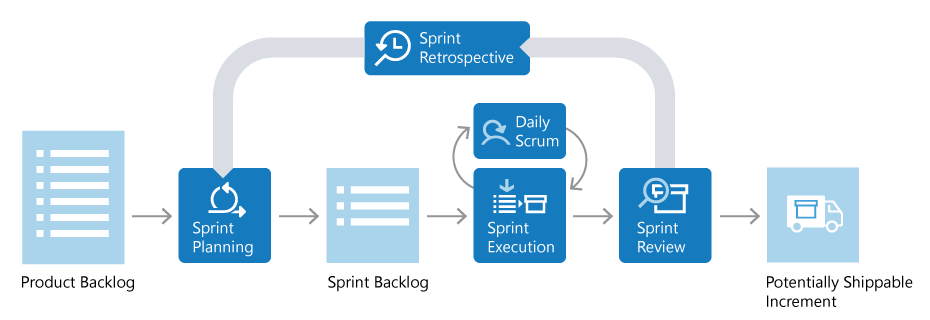
\includegraphics[scale=0.64]{imagenes/planificacion/agile-scrum-lifecycle-diagram.png}}
    \caption{Ciclo de vida iterativo de Scrum.}
    \label{fig:scrum_ciclo_vida}
\end{figure}
El ciclo de vida de Scrum (Figura \ref{fig:scrum_ciclo_vida}, extraída de microsoft learn\footnote{\url{https://www.scrum.org/}}) se basa en un enfoque iterativo e incremental que permite a los equipos adaptarse a los cambios y entregar productos de alta calidad en un tiempo reducido. Los principios de transparencia, inspección y adaptación son fundamentales para alcanzar los valores centrales de Scrum, la calidad, flexibilidad, mejora continua, compromiso, coraje, ritmo y responsabilidad. 
Una de las características principales de Scrum es su enfoque en ciclos de desarrollo cortos llamados \emph{sprints}. Estos sprints suelen tener una duración de una a cuatro semanas, durante los cuales se planifican, desarrollan, prueban y entregan incrementos de software funcionales. Cada sprint comienza con una reunión de planificación en la que el equipo selecciona un conjunto de tareas para ser completados durante el sprint. Podemos definir Scrum según los elementos que lo componen:

\begin{itemize}
    \item \textbf{Artefactos}
    \begin{itemize}
        \item \textbf{Product Backlog (Pila del producto)}: es una lista ordenada y priorizada de todas las funcionalidades, características y mejoras que podrían ser necesarias para el producto. Es responsabilidad del Product Owner y se actualiza constantemente a medida que se obtiene nueva información o se generan cambios en los requisitos.
        \item \textbf{Sprint Backlog (Pila del sprint)}: es un conjunto de elementos seleccionado del Product Backlog para el sprint. Se descomponen en tareas de desarrollo más pequeñas junto con estimaciones de tiempo, expresando los requisitos en lenguaje técnico.
    \end{itemize}
        

    \item \textbf{Reuniones}
    \begin{itemize}
        \item \textbf{Sprint Planning}: marca el inicio de cada sprint y se realiza con el propósito de identificar el objetivo principal del sprint y las tareas concretas que se van a desarrollar en él. Como resultado, se genera el Sprint Backlog.
        \item \textbf{Daily Meetings}: reunión diaria de unos 15 minutos donde participan los miembros del Equipo de Desarrollo y el Scrum Master. Es una manera de estar al tanto del trabajo realizado y cuáles son los siguientes pasos. Es una oportunidad de identificar rápidamente obstáculos o problemas.
        \item \textbf{Sprint Review}: al final del sprint se pone en común todo el trabajo realizado durante el Sprint. Sirve para recoger información o feedback sobre el estado del proyecto.
        \item \textbf{Sprint Retrospective}: el equipo dedica tiempo a reflexionar sobre los aspectos positivos y las áreas que requieren mejoras. Como resultado de la retrospectiva, se generan acciones específicas para implementar en el siguiente sprint.
    \end{itemize}

    \item \textbf{Roles}: representan responsabilidades dentro del proyecto.
    \begin{itemize}
        \item \textbf{Stakeholders}: son todos aquellos interesados en el proyecto, tanto personas como organizaciones (gente de marketing, comerciales, usuarios, etc).
        \item \textbf{Product Owner (PO, propietario)}: debe conocer perfectamente el entorno de negocio del cliente, las necesidades y el objetivo que se persigue con el sistema que se está construyendo. Debe conocer también como funciona Scrum para desempeñar bien su rol. Su responsabilidad principal es la de crear, administrar, y priorizar el P.Backlog, así como validar o rechazar el incremento resultado de cada iteración.
        \item \textbf{Scrum Master (director del proyecto)}: garantiza el correcto funcionamiento de los procesos y metodologías que se empleen en el equipo. Gestiona el proceso e intenta mejorar la productividad del equipo. Promueve los valores y prácticas de Scrum, elimina impedimentos, facilita la colaboración entre los roles, actúa como escudo ante cosas externas. Se asegura de que el PO sepa cómo ordenar la pila de producto para maximizar el valor generado en cada sprint.
        \item \textbf{Equipo de desarrollo}: es el que se encarga de desarrollar el producto y hacer los entregables en incrementos. Los miembros del equipo necesitan ser auto-organizados, multidisciplinares, multifuncionales, con un alto compromiso y sin jerarquías internas. Son los verdaderos responsables de que el producto salga adelante y se completen los incrementos. Se encargan de estimar el tamaño de los ítems del backlog. Es importante que el equipo de desarrollo comprenda bien la visión que tiene el PO acerca del producto. Suelen estar formados de entre 5 a 9 personas.
    \end{itemize}
\end{itemize}

\subsection{XP}
La programación extrema (XP) es una metodología ágil que se centra en la velocidad y la simplicidad con ciclos de desarrollo muy cortos. En XP se promueven una serie de valores: comunicación, simplicidad, retroalimentación, coraje y respeto. Diseñada para entornos dinámicos con requisitos cambiantes y orientado fuertemente hacia la codificación, reduciendo considerablemente la documentación. En XP, las tareas que se terminan son susceptibles de ser modificadas durante el transcurso del proyecto, incluso después de que funcionen correctamente, por lo que son importantes las siguientes prácticas.

\begin{itemize}
    \item \textbf{Prácticas}: XP propone una serie de prácticas a nivel técnico que se deberían adoptar para el desarrollo del proyecto \cite{extremeXP_Page}. Las más importantes a mi parecer son:
    \begin{itemize}
        \item \textbf{Programación a pares}: los programadores trabajan en parejas, mientras uno escribe el código, el otro proporciona comentarios y realiza revisiones en tiempo real. Esto promueve el intercambio de conocimientos, la revisión de código constante y la minimización de errores.
        \item \textbf{Propiedad colectiva del código}: la propiedad colectiva anima a todos a aportar nuevas ideas sobre todos los segmentos del proyecto. Cualquier desarrollador puede cambiar cualquier línea de código para añadir funcionalidad, corregir errores, mejorar diseños o refactorizar.
        \item \textbf{Estándares de codificación}: el código ajustarse a las normas de codificación acordadas. Estas hacen que el código sea consistente y fácil de leer y refactorizar para todo el equipo. Un código con el mismo aspecto o que sigue unas normas fomenta la propiedad colectiva.
        \item \textbf{Marcha sostenible}: encontrar un ritmo de trabajo para el equipo de desarrollo donde todos los miembros se sientan cómodos. Las horas extra acaban con el espíritu y la motivación del equipo. A veces, menos es más.
        \item \textbf{Integración continua}: los equipos de XP no esperan a que se completen las iteraciones, sino que se integran constantemente. Se cuenta con un repositorio de código donde los desarrolladores envían el código cada poco tiempo.
        \item \textbf{Refactorización}: reescribir ciertas partes del código para aumentar su legibilidad y mantenibilidad pero sin modificar su comportamiento. Las pruebas han de garantizar que en la refactorización no se ha introducido ningún fallo. Evita la complejidad innecesaria.
        \item \textbf{Desarrollo orientado a pruebas}: las pruebas son frecuentemente repetidas y automatizadas cada vez que se haga un cambio, por pequeño que sea, antes de desplegar la nueva versión. Se suelen escribir antes que el propio código.
    \end{itemize}
    
    \item \textbf{Roles}
    \begin{itemize}
        \item \textbf{Programador}: encargados de escribir y probar el código.
        \item \textbf{Cliente}: representa los intereses del usuario y es responsable de proporcionar las necesidades, requisitos del software y establecer prioridades. 
        \item \textbf{Entrenador (Coach)}: es el líder del equipo, actúa como facilitador y promotor de las prácticas y valores de XP, y ayuda al equipo a mejorar y adaptarse.
        \item \textbf{Consultor}: miembro externo al equipo de desarrollo con conocimiento específico en un tema necesario.
        \item \textbf{Rastreador (Tracker)}: se encarga de gestionar la planificación y llevar un seguimiento del proyecto detectando los problemas en él.
    \end{itemize}
\end{itemize}

\subsection{Aplicación de Scrum/XP al proyecto}

Algunas de las características y prácticas mencionadas de cada una de las metodologías no son aplicables al proyecto dada su naturaleza e integrantes, como por ejemplo, la programación por parejas propia de XP. Se describe ahora, el enfoque que se le ha dado del híbrido Scrum/XP al proyecto.

Se lleva a cabo una planificación por \emph{Sprints} de entre 2 a 4 semanas, dependiendo de las tareas a realizar. Entre medias y al final de cada sprint, se agendará una \emph{reunión con la tutora} en la que se hará retrospectiva del mismo, para comprobar el estado y avance del proyecto. Se revisará qué se ha hecho durante el sprint y cómo se ha hecho, repasando las novedades desde la última iteración y puntos a mejorar o pulir, priorizando las siguientes tareas a realizar en base a los resultados. Igualmente, se mantendrá el contacto con el tutor de manera constante vía correo electrónico.


Mediante la \emph{integración continua}, los cambios se envían con frecuencia a un repositorio compartido con un sistema de control de versiones. Cada vez que se realiza un cambio o se desarrolla una nueva funcionalidad, se ejecutan \emph{pruebas} en el dataset completo de moléculas, comprobando rápidamente si los resultados son los esperados (parcial o totalmente), y detectar cualquier error antes de que se convierta en un problema más grave. Se sigue por tanto un \emph{desarrollo incremental}, añadiendo pequeñas funcionalidades o porciones de código funcional, centrándome en un aspecto específico en cada commit subido a github.

Se asignarán los roles propios de Scrum. El papel de \emph{Equipo de desarrollo} recae sobre el estudiante, y al ser únicamente una persona, también actuará como \emph{Scrum Master} siendo responsable de la correcta aplicación de la metodología y prácticas al proyecto. La tutora actuará como \emph{Product Owner}, conoce las necesidades del proyecto y el dominio del problema, hace de intermediaria con el cliente y ayuda al equipo de desarrollo a priorizar las tareas. Como posibles clientes o personas interesadas (\emph{stakeholders}) podemos incluir al grupo de investigación del ICIQ, con el que se mantiene el contacto frecuentemente a través del Product Owner.

Al ser OpenBabel una librería existente es importante mantener unos \emph{estándares de codificación} y un estilo consistente. Teniendo eso en mente, y usando el \emph{Refactoring}, se realizan cambios manteniendo el código limpio y legible. Se han usado las guías propias de OpenBabel y la documentación oficial orientada a desarrolladores para añadir nuevas funcionalidades \footnote{\url{https://openbabel.org/docs/current/OpenBabel.pdf}}, \footnote{\url{https://acortar.link/Openbabel_Adding_Plugins}}. Además, se busca ante todo la simplicidad a la hora de programar, evitando añadir funcionalidades extremadamente complejas o innecesarias y la adopción de soluciones sencillas.

\section{Planificación}
Inicialmente se elaboró una planificación estimada general sin mucho detalle, dividida en bloques grandes de trabajo, para establecer marcos de tiempo y controlar el ritmo del proyecto. Se puede ver en la Figura \ref{fig:gantt_incial_estimado}
\begin{figure}[h!]
    \centering
    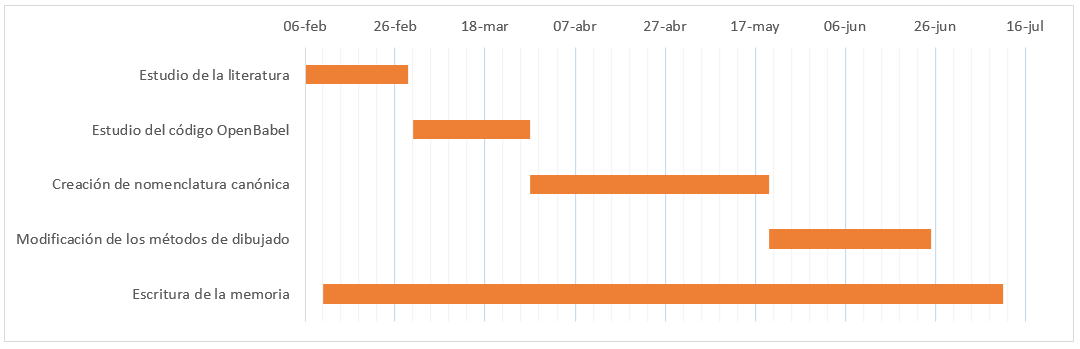
\includegraphics[scale=0.32]{imagenes/planificacion/planificacion_estimada.png}
    \caption{Diagrama de Gantt sobre la planificación inicial estimada}
    \label{fig:gantt_incial_estimado}
\end{figure}

Conforme se iba profundizando en el dominio del problema y entendiendo más sobre la problemática, se fueron subdividiendo y priorizando las tareas. A continuación, se desglosan las tareas definidas para el proyecto, separados en sprints: 

\begin{itemize}
    \item \textbf{Bloque 1}: Investigación y aprendizaje previo. Estudio del estado del arte.
    \begin{itemize}
        \item Lectura artículos y publicaciones sobre Chemoinformatics
        \item Repaso de química general y estudio de química organometálica
        \item Experimentación y pruebas iniciales con distintas herramientas
    \end{itemize}

    \item \textbf{Bloque 2}: Estudio del paquete OpenBabel
    \begin{itemize}
        \item Lectura detallada del código OpenBabel
        \item Experimentación moléculas usando el dibujado de OpenBabel
    \end{itemize}

    \item \textbf{Bloque 3}: Proceso de mejora del sistema de dibujado
    \begin{itemize}
        \item Detección de estructuras de ciclopentadienilo (Cp)
        \item Modificación dibujado moléculas con Cp individuales
        \item Detección de múltiples Cp en la misma molécula usando bloques
    \end{itemize}

    \item \textbf{Bloque 4}: Creación de nomenclatura canónica
    \begin{itemize}
        \item Detección de bloques en el SMILES y creación del árbol genérico
        \item Desarrollo del algoritmo canónico para moléculas con 1 metal
        \item Algoritmo canónico para moléculas con 2 o más metales
    \end{itemize}

    \item \textbf{Bloque 5}: Documentación del proyecto
    \begin{itemize}
        \item Redacción de la memoria
    \end{itemize}
\end{itemize}


\begin{landscape}

En el siguiente Diagrama de Gantt (Figura \ref{fig:gantt_real}) se presenta la planificación real del proyecto:

    \begin{figure}[h!]
        \centering
        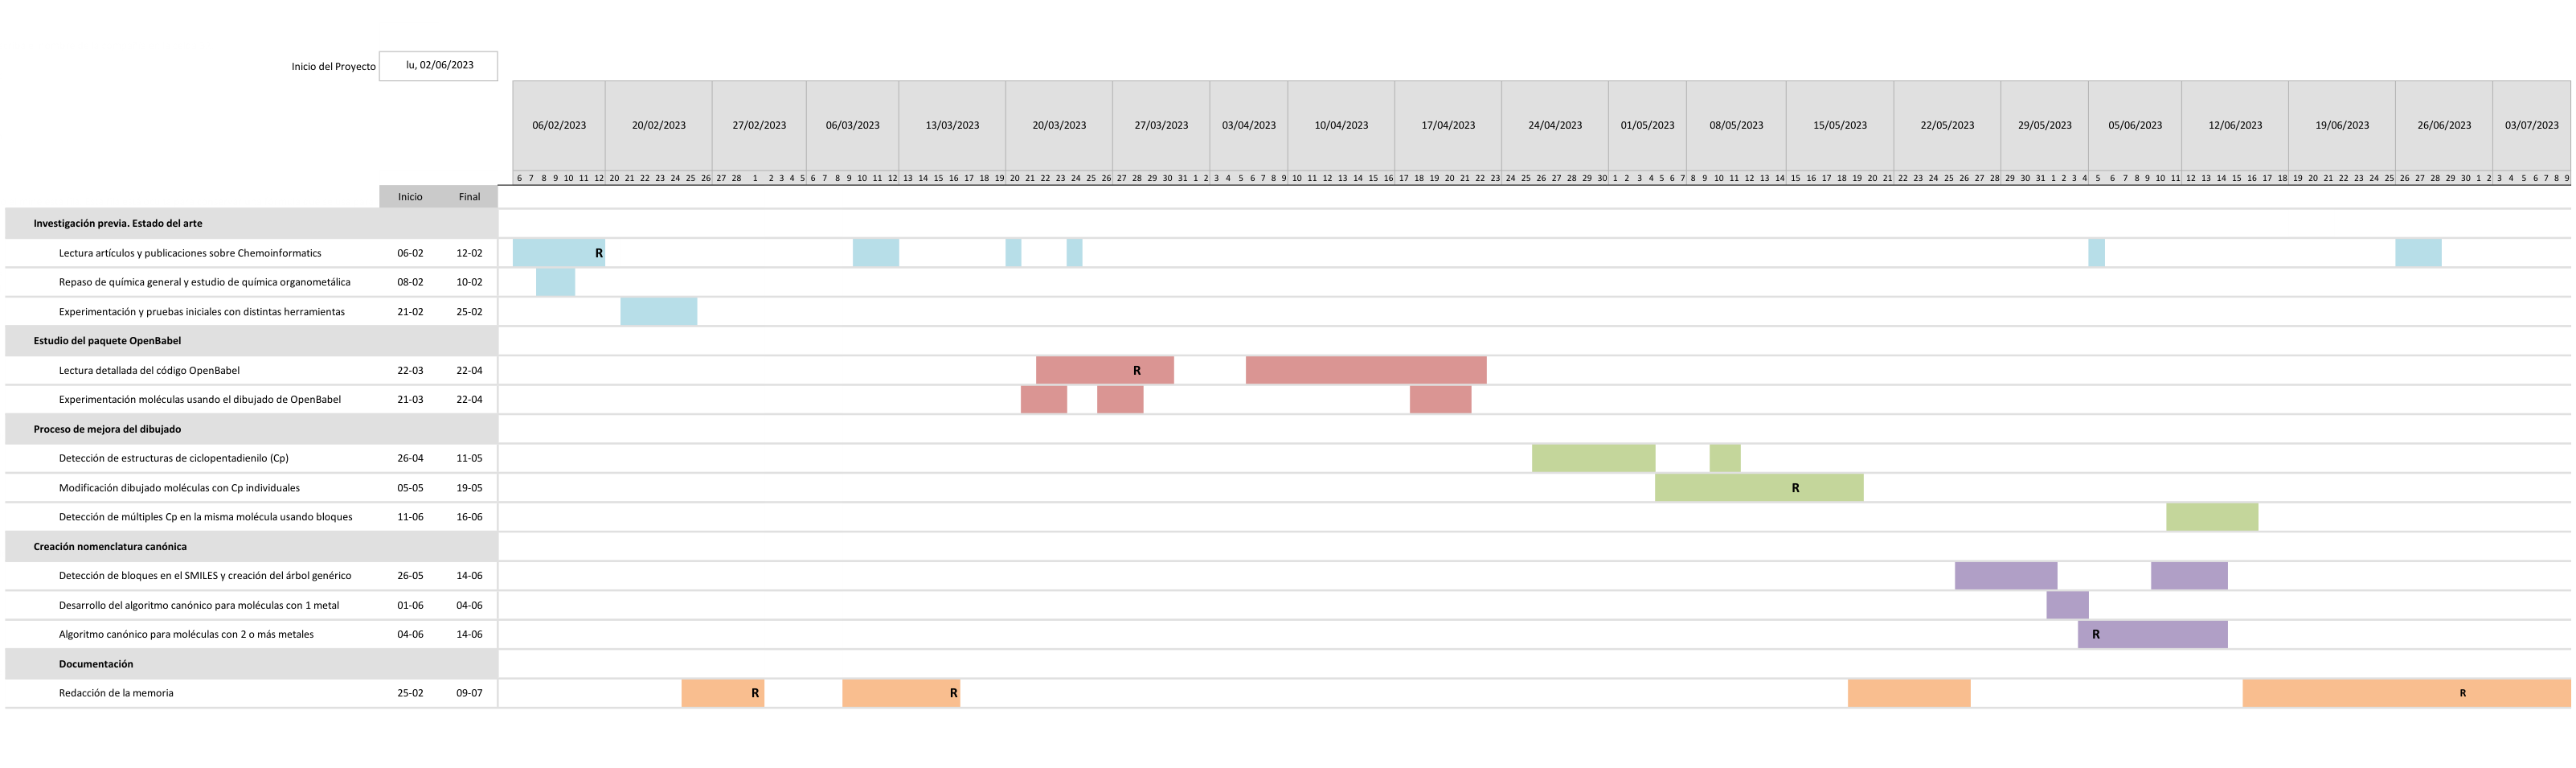
\includegraphics[scale=0.9]{imagenes/planificacion/planificacion_real.png}
        \caption{Diagrama de Gantt sobre la planificación temporal real}
        \label{fig:gantt_real}
    \end{figure}
\end{landscape}

% 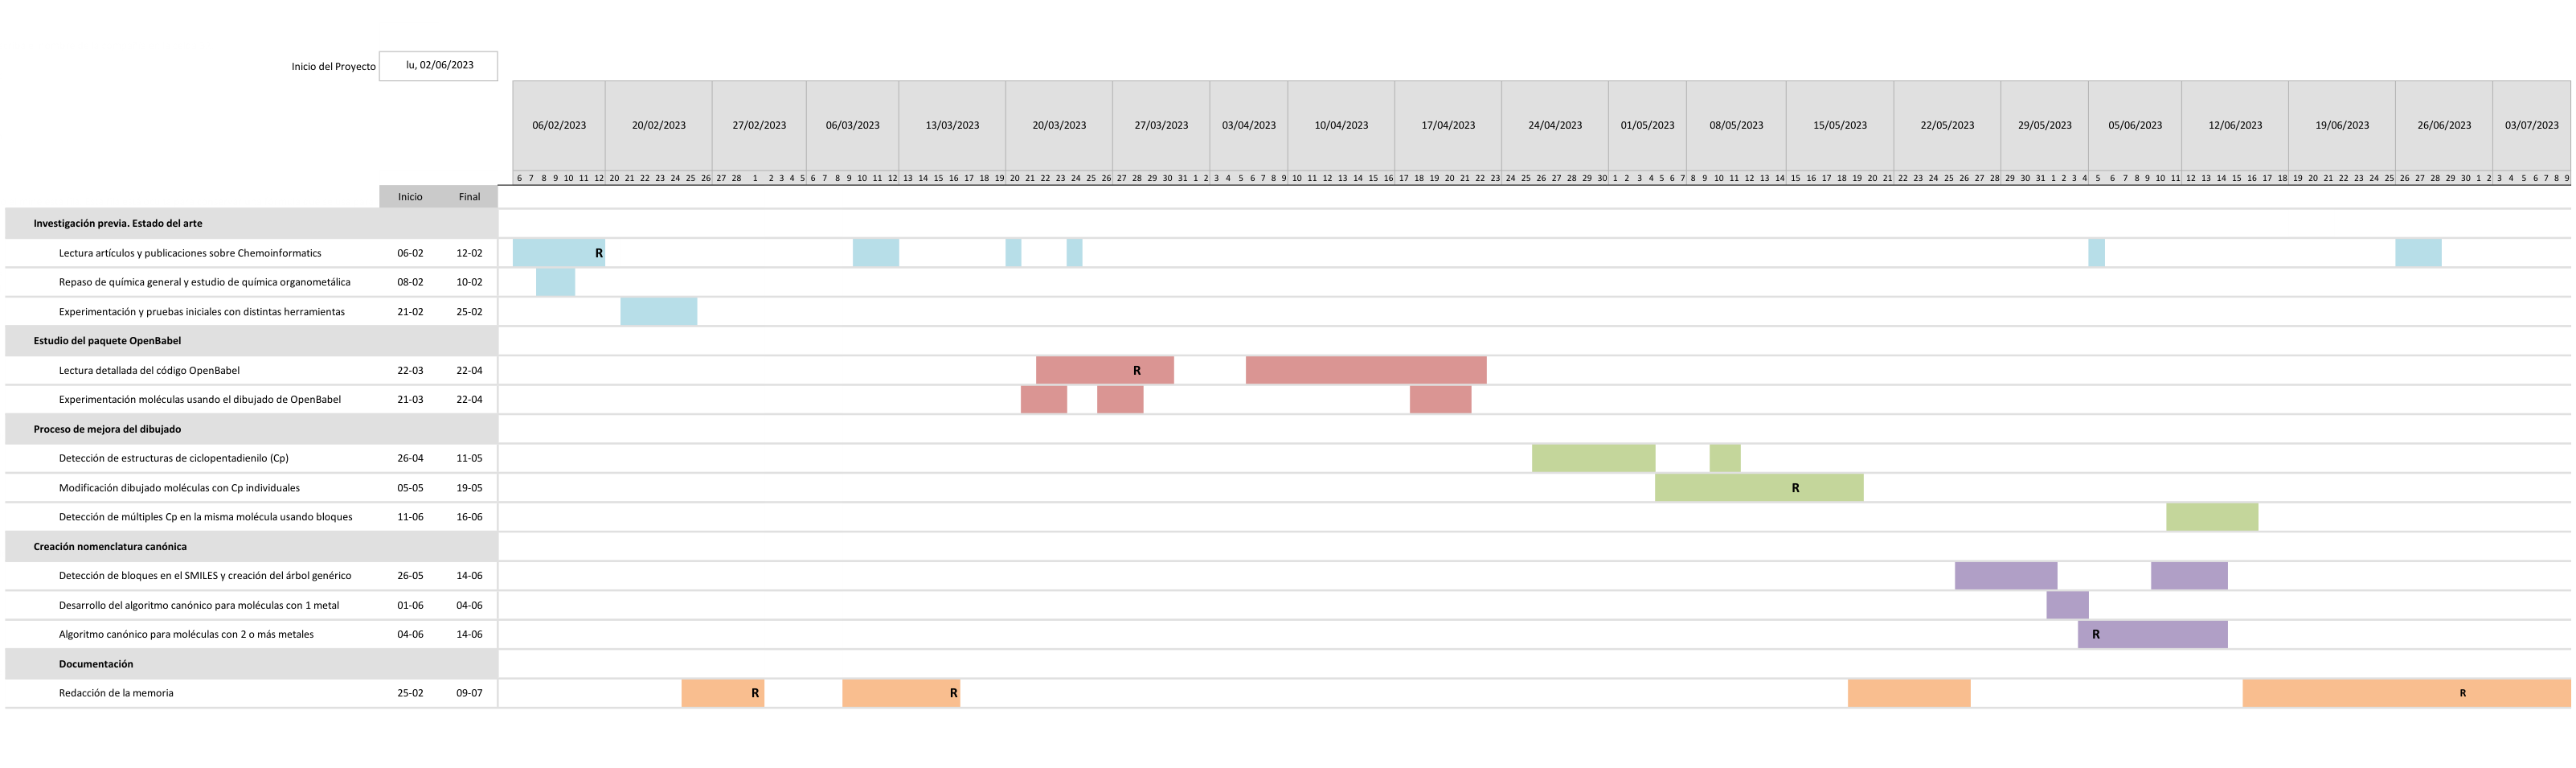
\includepdf[pages=-, offset=0 0,landscape=true,]{imagenes/planificacion/planificacion_real.png}


Como describo en la Sección \ref{riesgos_materializados}, el proceso de compresión del código base se alargó más de lo esperado, retrasando un poco el resto de tareas. En contraparte, la canonización y dibujado de las moléculas me llevó menos tiempo del estimado. Además, se invirtió el orden entre la modificación del sistema de dibujado y la creación del algoritmo de canonización con respecto a la planificación inicial. A priori era más sencillo alterar esa parte del código, y se podían obtener resultados más visuales.

\section{Gestión de la configuración}
En este apartado se describirá cómo se ha llevado a cabo la gestión de los activos de este proyecto, es decir, el código desarrollado y la documentación generada. Dado que son partes fundamentales del trabajo, atendiendo al análisis de riesgos descrito en la sección \ref{riesgos} y el plan de actuación frente a la pérdida de información, se detalla a continuación la gestión de ambas.

\subsection{Gestión del código}
Para la gestión del código se ha usado un control de versiones a través de Git y Github. Ambas herramientas en conjunto permiten ir creando versiones intermedias del código conforme se va desarrollando y hacer copias de seguridad en la nube. También son muy útiles para proyectos colaborativos, donde varias personas del equipo pueden combinar fácilmente su parte del código desarrollado y revisar el progreso subido hasta el momento.
El procedimiento a seguir en la mayoría de casos es bastante similar. Se creará un repositorio remoto en la plataforma de GitHub con el nombre de \emph{TFG} —o el que uno prefiera— donde se irán almacenando los cambios\footnote{\url{https://github.com/Jesnm01/TFG}}. En la carpeta de trabajo local de nuestra computadora, carpeta que contendrá en mi caso todos los elementos de los que quiera llevar un control, se creará un repositorio local usando Git, que habrá que vincular con el remoto para poder ir sincronizando los cambios. 


\subsection{Gestión de la documentación}
En lo relativo a la documentación, el proceso de gestión será similar ya que también se ha usado GitHub para su control de versiones. Esta se ha redactado en LaTeX usando el servicio online Overleaf. Overleaf cuenta con una opción para sincronizar el proyecto con un repositorio de GitHub, pero es una opción de pago. En su lugar, descargo el proyecto en el repositorio local y desde ahí ya realizo dicha sincronización para subir los cambios en el remoto.

Además, dada la naturaleza del proyecto y de la metodología de desarrollo utilizada, se ha llevado un registro de las reuniones con la tutora que también se ha ido actualizando periódicamente. Este documento pretende recoger los contenidos más relevantes de las reuniones: preguntas, comentarios, anotaciones, tareas que hacer, cosas pendientes de una reunión a otra, revisiones, y puntos a mejorar, entre otras cosas.



\section{Gestión de recursos} \label{gestion_recursos}

\subsection{Recursos humanos}
\begin{itemize}
    \item \textbf{Dña. Rocío Celeste Romero Zaliz}, profesora del Departamento de Ciencias de la Computación e Inteligencia Artificial de la Universidad de Granada en calidad de tutora del proyecto. A cargo de la supervisión y guía del alumno durante su desarrollo del trabajo.
    \item \textbf{Jesús Navarro Merino}, estudiante del grado en Ingeniería Informática en la Escuela Técnica Superior de Ingenierías Informática y Telecomunicación.
\end{itemize}


\subsection{Recursos materiales}
Para este proyecto no se han necesitado recursos adicionales, habiéndose usado únicamente los siguientes recursos materiales, ya existentes: 
\begin{itemize}
    \item \textbf{Portátil personal}: Portátil ACER Aspire A515-51G-8907 con un procesador Intel Core i7 8550U 1.8GHz, 20GB de memoria RAM y una arquitectura de 64 bits. Se ha usado durante todo el proyecto, para labores de programación y redacción de la memoria.
    \item \textbf{Pantalla}. Monitor utilizado de apoyo a la pantalla propia del portátil. De la marca AOC, de 24 pulgadas con una resolución de 1920x1080.
\end{itemize}


\subsection{Recursos software} \label{recursos_software}
En esta sección describiré todas aquellas herramientas software empleadas durante la realización del proyecto. Todas y cada una de ellas son herramientas de software libre, gratuitas o disponibles a través de licencias de estudiantado. A continuación se lista el software usado:
\begin{itemize}
    \item \textbf{Sistema operativo}: Windows 10 Home. Aunque por lo general Windows no es gratuito, al estar utilizando la típica licencia OEM que trae preinstalada el ordenador al comprarlo, la considero como tal.
    
    \item \textbf{Visual Studio C++}: es un IDE muy potente de Microsoft orientado a crear aplicaciones .NET y C++ para Windows. Se ha usado su versión gratuita Visual Studio Community 2022. Permite editar, depurar, realizar pruebas de testing, además de tener control de versiones integrado, entre otras cosas. Aquí se ha llevado a cabo todo el desarrollo del código.
    
    \item \textbf{OpenBabel}: Open Babel es una biblioteca de código abierto multiplataforma utilizada en química computacional y ciencias relacionadas para la conversión y manipulación de estructuras químicas en varios formatos. He trabajado con la versión 3.1.1 disponible en su repositorio de GitHub oficial\footnote{\url{https://github.com/openbabel/openbabel}}.

    \item \textbf{CMake}: es una herramienta de generación de archivos de compilación que simplifica el proceso de compilación y construcción de proyectos, permitiendo una configuración flexible e independiente de la plataforma. CMake utiliza archivos de configuración llamados CMakeLists.txt para describir la estructura del proyecto y las dependencias necesarias. Se ha usado en su versión 3.25.2 para la compilación y creación de soluciones de OpenBabel.

    \item \textbf{Git}: software de código abierto para el control de versiones de un proyecto.
    \item \textbf{Github}: es una plataforma donde se alojará el código y la documentación del proyecto. Utiliza Git por debajo y es una de las plataformas gratuitas para alojamiento de código mas empleadas a nivel mundial.

    \item \textbf{Google Colab}: es una plataforma en línea gratuita ofrecida por Google que permite a cualquier usuario escribir y ejecutar código en el navegador. Es una herramienta basada en la nube que proporciona un entorno de ejecución como si fueran notebooks de Jupyter, es decir, se puede escribir, editar y ejecutar código en bloques/celdas interactivos. Se ha usado durante las etapas iniciales del proyecto para la experimentación con diversas moléculas.
    
    \item \textbf{Zotero}: software de gestión de referencias bibliográficas que permite recopilar, organizar, citar y generar fácilmente una bibliografía en varios estilos de formato estándares según los documentos, páginas webs, artículos o archivos PDF guardados. Facilita la creación de referencias y citas en documentos académicos, ahorrando tiempo y asegurando un uso correcto de las fuentes consultadas.
    
    \item \textbf{Google Meet}: servicio de videoconferencias de Google. Plataforma utilizada para las reuniones con la tutora.

    \item \textbf{Google Drive Sync}: ahora llamada Google Drive para PC, es una aplicación de Google que permite sincronizar los archivos y carpetas de la computadora con la cuenta de Drive. Usado para realizar copias de seguridad —adicionales a lo almacenado en GitHub— de algunos archivos importantes. 

    \item \textbf{Overleaf}: herramienta online para la redacción de documentos en LaTeX usada para la documentación de este proyecto.

    \item \textbf{Clockify}: herramienta online que te permite registrar las horas dedicadas a un proyecto.

    \item \textbf{Umbrello}: herramienta que combina funciones de modelado y generación de código para el lenguaje unificado de modelado (UML). Usado para la elaboración de los diagramas de clases.

    \item \textbf{Correo UGR}: servicio de correo electrónico institucional de la UGR.

    \item \textbf{Microsoft Word}: procesador de textos de Microsoft usado para apuntes personales y documentación en sucio. Disponible a través de la cuenta de Microsoft Office 365 que ofrece la universidad.

    \item \textbf{Microsoft Excel}: utilizado para la creación de algunas tablas y gráficos incluidos en la memoria. Disponible a través de la cuenta de Microsoft Office 365 que ofrece la universidad.

    \item \textbf{Visual Studio Code y LaTeX}: VSCode es un editor de texto, que a través de algunas extensiones, permite editar, compilar y visualizar ficheros LaTeX. Es la alternativa a Overleaf según lo descrito en la Sección \ref{riesgos}. 

    
    
\end{itemize}

\section{Gestión de costes}
\textbf{TERMINAR esto cuando vaya acabando el trabajo}

En esta sección se realizará una estimación de los costes asociados al proyecto, atendiendo a los recursos descritos en la Sección \ref{gestion_recursos}. La elaboración de un presupuesto preciso en muchos casos puede suponer un desafío, ya que los proyectos software a menudo están sujetos a cambios y variables imprevistas, pero es una tarea importante para estudiar su viabilidad. 

\subsection{Coste de recursos humanos}
Si actuáramos como una empresa en un proyecto software al uso, existen muchos componentes que tener en cuenta para montar esta sección del presupuesto. Aspectos como el salario de los trabajadores y compensaciones varias, el coste de los procesos de selección y contratación, formación y desarrollo del personal, costes laborales adicionales (seguros, vacaciones, etc), o costes de personal externo (consultores o subcontratistas) entre otras cosas.
Dada la naturaleza de este proyecto, en relación a los gastos asociados a recursos humanos contamos con un equipo de desarrollo formado por una persona que tendrá el papel de Ingeniero Informático. Para estimar el costo de su trabajo, se indica el número total de horas dedicadas.

El intervalo de tiempo que está pensado para el proyecto son 5 meses, desde febrero hasta junio. 

\begin{center}
    $Dias\ totales\ =\ 5\ meses\ *\ 30\ dias / mes\ =\ 150\ dias$    
\end{center}

A este tiempo hay que descontarle los días no laborables de fines de semana más los días de vacaciones correspondientes por mes trabajado:

\begin{equation*}
    \textit{Dias no laborables} = \left( \frac{8 \textit{dias}}{mes} + \frac{22 \textit{ dias vacaciones}}{12 \textit{ meses}}\right) * 5 \textit{ meses} \approx 50 \textit{ dias}
\end{equation*}

Eso nos deja un total de 100 días aproximadamente de trabajo. Teniendo en cuenta una media semanal de 30 horas trabajadas repartidas en 6 horas diarias, tendríamos el siguiente total de horas trabajadas:
\begin{equation*}
    \textit{Horas trabajadas} = 100 \textit{dias} * 6 \textit{ horas/dia} = 600 \textit{ horas}
\end{equation*}

Esta cifra duplicaría la cantidad de horas que le corresponderían a un TFG según sus créditos asignados por la universidad. Estos cálculos como tal serían una estimación, pero se ha utilizado durante el desarrollo del proyecto la herramienta Clockify para el registro real de las horas dedicadas. Como se ve en la figura \ref{fig:clockify}, han sido \textbf{XXXXX} horas en total,
por lo que usaré ese dato para calcular el coste.

\begin{figure}[h!]
    \centering{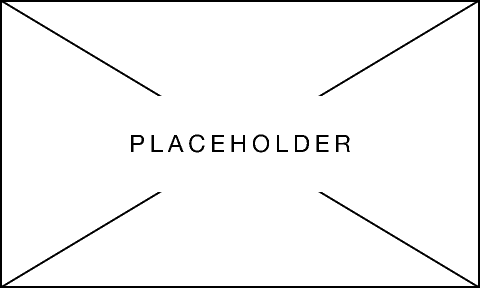
\includegraphics[scale=0.4]{imagenes/placeholder.png}}
    \caption{Registro de horas dedicadas al proyecto a través de Clockify}
    \label{fig:clockify}
\end{figure}

Según varias fuentes\footnote{\url{https://www.jobted.es/salario/ingeniero-informático}}\footnotecomma\footnote{\url{https://acortar.link/infojobs_salario}}\footnotecomma\footnote{\url{https://acortar.link/uax_salario}}, el salario medio de un ingeniero informático recién graduado está en torno a 21.000€. Siendo equivalente, unos 1750€ mensuales, que son 13,46€/hora. Con todo eso, tenemos que:
\begin{equation*}
    \textit{Coste total recursos humanos} = XXXX \textit{horas} * 13,46\EUR{}/hora = XXX \EUR{}
\end{equation*}


\subsection{Costes de recursos materiales}

Dado que no se han adquirido expresamente para este proyecto, ya que se poseían con anterioridad, no se valora su precio de compra como tal sino su valor de depreciación. Los productos electrónicos experimentan un proceso llamado depreciación, que conlleva una devaluación gradual a lo largo de su vida útil. Es importante tener esto en cuenta para estimar su valor actual y el coste del recurso. Esta estimación refleja el valor de un activo desde un punto de vista contable.

Al referirnos a la depreciación de un activo a lo largo de su vida útil, no se incluyen situaciones en las que sufra daños debido a accidentes, desastres naturales u otros eventos similares. En cambio, estamos hablando del desgaste del uso cotidiano, así como los impactos derivados de las innovaciones tecnológicas que surgen durante ese período que puedan dejar obsoleto el dispositivo.

Para calcular el valor actual de los activos utilizaré el método de depreciación lineal, que considera un desgaste uniforme durante su uso, mostrando el resultado del gasto anual de depreciación\cite{depreciacion_pcs}. Necesitamos lo primero, hallar el valor residual del activo, es decir, el valor que se estima que tendrá cuando llegue al final de su vida útil. Usaré para los dispositivos electrónicos una vida útil de 8 años. Haré un ejemplo con el coste del portátil.

\begin{equation*}
    \textit{Valor residual} = {\frac{\textit{Coste inicial}}{\textit{Vida util (años)}}} = \frac{689 \EUR{}} {8 \textit{ años}} = 86,125 \EUR{}
\end{equation*}

Con el valor residual estimado, se puede calcular la depreciación lineal anual con la siguiente fórmula.

\begin{equation*}
    \textit{Depreciación} = {\frac{\textit{Coste inicial} - \textit{Valor residual}}{\textit{Vida util (años)}}} = \frac{689\EUR{}-86,125\EUR{}} {8 \textit{ años}} = 75,36 \EUR{}
\end{equation*}

Teniendo estos 2 datos, se puede calcular el valor actual del activo teniendo en cuenta sus años de antigüedad. Se muestran todos los datos relativos a los costes materiales en la Tabla \ref{tabla:costes_materiales}.


\begin{table}[ht]
\small
    \begin{tabular}{lllll}
    \toprule 
    % Al parecer tengo que hacer esto asi tan extraño (meter una tabla de 1 celda dentro de la propia celda para poder meter un salto de linea...)
    \textbf{Recurso} & \textbf{\begin{tabular}[c]{@{}l@{}}Valor\\ inicial (€)\end{tabular}} & \textbf{\begin{tabular}[c]{@{}l@{}}Depreciación\\ anual (€)\end{tabular}} & \textbf{\begin{tabular}[c]{@{}l@{}}Antigüedad\\ (años)\end{tabular}} & \textbf{\begin{tabular}[c]{@{}l@{}}Valor\\ actual (€)\end{tabular}} \\ 
    \midrule
    Portátil personal           & 689 & 75,36 & 5 & 312,2         \\ 
    Pantalla AOC                & ~230 & 25,15 & 2 & 179,69         \\ 
    \midrule
    \multicolumn{4}{r}{\textbf{Total:} } & 491,89 \\
    \bottomrule
\end{tabular}
\caption{Tabla de los costes materiales}
\label{tabla:costes_materiales}
\end{table}

\subsection{Costes software}
Los costes relacionados con los recursos software son nulos. Como indico en el listado de recursos de la Sección \ref{recursos_software}, son herramientas de software libre o utilizadas mediante licencias gratuitas, por lo que no suponen coste alguno en el desarrollo de este proyecto.

\subsection{Otros costes}
Aquí se incluyen todos los demás gastos que han sido necesarios para el desarrollo del proyecto y que no pertenecen a los apartados anteriores. Principalmente son los gastos vinculados a las facturas de la luz e Internet. El coste de la tarifa de Internet contratada es de 40€/mes, que a lo largo de los 5 meses el total asciende a 200€. Para la luz, una estimación posible serían 19,58€, teniendo en cuenta el gasto que suponen los recursos materiales en base a una factura trimestral de 11,80€.

\begin{table}[ht]
    \centering
    \begin{tabular}[t]{lc}
        \toprule
        \textbf{Recursos} & \textbf{Importe (€)}  \\
        \midrule
        Luz         &   19,58   \\
        Internet    &   200      \\
        \bottomrule
    \end{tabular}
    \caption{Tabla de costes adicionales}
    \label{tabla:costes_adicionales}
\end{table}




\subsection{Presupuesto final}
Se presenta por tanto el presupuesto completo asociado al proyecto, dividido en cada una de las secciones tratadas anteriormente. Se ve el desglose en la Tabla \ref{tabla:presupuesto_total}.
\begin{longtable}[c]{lm{2cm}r}
\toprule
\textbf{Detalle}                        && \textbf{Importe} \\
\endfirsthead
%
\endhead
%
% \hline
\endfoot
%
\endlastfoot
%
\midrule
                                        % &                 \\\hline
\textbf{Costes de recursos humanos}     && \textbf{X €} \\
Trabajo autónomo                        && X €          \\
\midrule
\textbf{Costes de recursos materiales}  && \textbf{491,89 €} \\
Portátil personal                       && 312,2 €            \\ %Esto para darle un tabulado al elemento
Pantalla de apoyo                       && 179,69 €             \\ 
\midrule
\textbf{Costes de recursos software}    && \textbf{0,00 €}    \\
                                        % & \multicolumn{1}{l}{}    \\
Windows 10                              && 0,00 €             \\
Visual Studio C++                       && 0,00 €             \\
OpenBabel                               && 0,00 €             \\
CMake                                   && 0,00 €             \\
Git                                     && 0,00 €             \\
GitHub                                  && 0,00 €             \\
Google Colab                            && 0,00 €             \\
Zotero                                  && 0,00 €             \\
Google Meet                             && 0,00 €             \\
Google Drive Sync                       && 0,00 €             \\
Overleaf                                && 0,00 €             \\
Clockify                                && 0,00 €             \\
Correo UGR                              && 0,00 €             \\
Microsoft Word                          && 0,00 €             \\
Microsoft Excel                         && 0,00 €             \\
Visual Studio Code y LaTeX              && 0,00 €             \\
\midrule
\textbf{Costes adicionales}             && \textbf{219,58 €}  \\
                                        % & \multicolumn{1}{l}{}                   \\
Internet                                && 40€ x 5 meses = 200€           \\
Factura de la luz                       && 19,58 €            \\
                                        % & \multicolumn{1}{l}{}                   \\
\midrule
  &   \multicolumn{1}{r}{\textbf{Total:}} & \textbf{X €} \\
\bottomrule
\caption{Presupuesto total del proyecto}
\label{tabla:presupuesto_total}
\end{longtable}


\section{Análisis de riesgos} \label{riesgos}
El análisis de riesgos desempeña un papel fundamental en la planificación y ejecución exitosa de proyectos. A veces surgen imprevistos que pueden afectar en mayor o menor medida a la correcta evolución de estos. Por ello, la aplicación de este proceso resulta esencial para minimizar la incertidumbre, intentar evitar la aparición de esos riesgos, y en caso de que se materialicen, paliarlos o mitigarlos de manera efectiva mediante unos planes de actuación.

En este aparatado por tanto, se analizarán los riesgos potenciales del proyecto, incluyendo sus causas y el plan de acción para resolverlos o mitigar su impacto al máximo (Figura \ref{tabla:tabla_riesgos}). Además, se realizará una evaluación de la probabilidad de ocurrencia y del impacto asociado a cada riesgo, que se puede ver en la Figura \ref{tabla:riesgos_matriz_probabilidad}. Esto se basa en una matriz con 2 dimensiones: la probabilidad de ocurrencia de un riesgo y el impacto que tendría en el proyecto si se materializa. Se valorarán los riesgos según aspectos técnicos, de recursos humanos o complejidad y naturaleza del proyecto, y preguntas del tipo, ¿qué tan difícil sería recuperarse del riesgo?, ¿cuál es el resultado más negativo que podría originarse como consecuencia? o ¿ha sucedido este riesgo o alguno similar anteriormente?

\begin{figure}
    \centering
    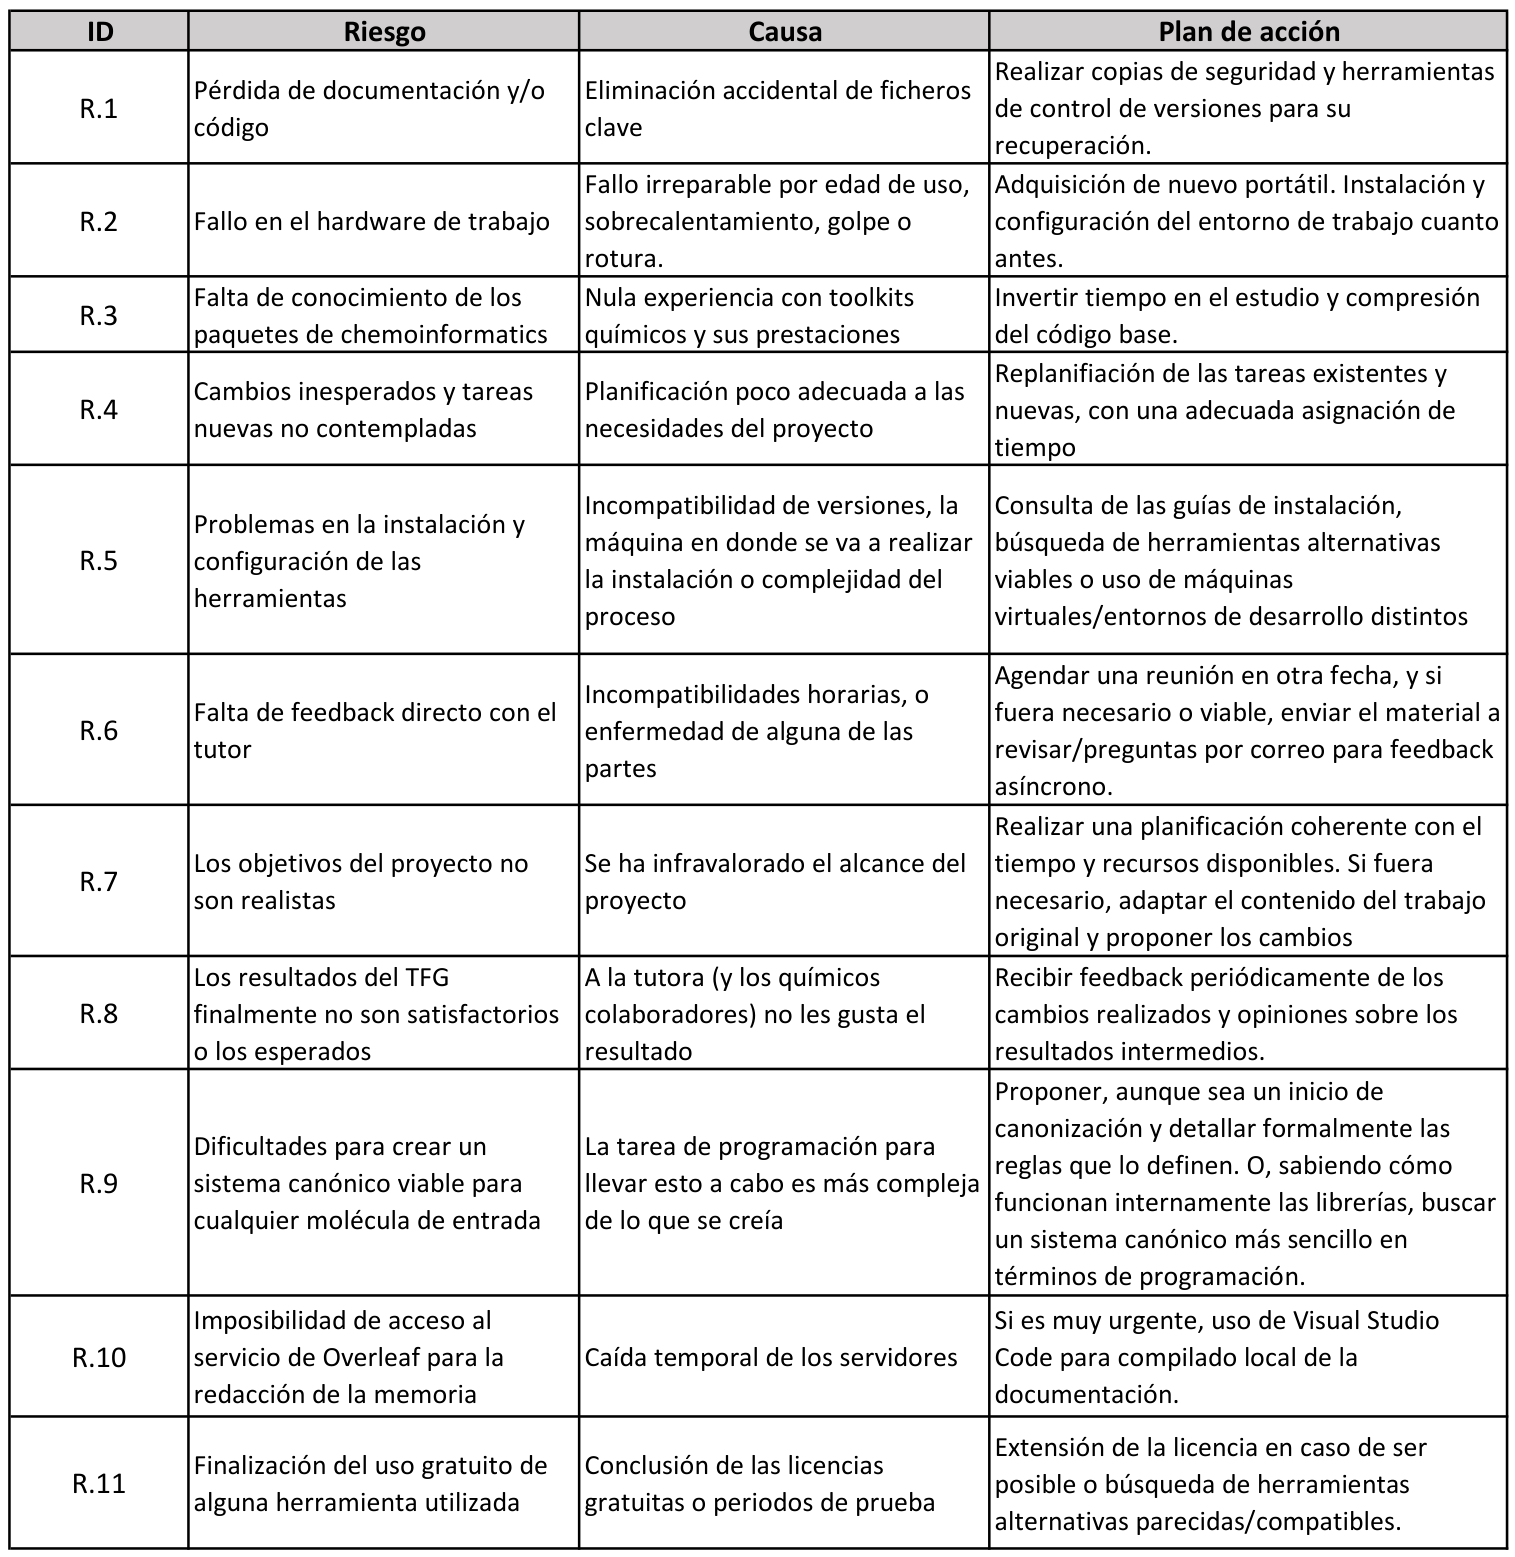
\includegraphics[scale=1]{imagenes/planificacion/riesgos-1_cropped.png}
    \caption{Riesgos del proyecto, causas, y planes de actuación}
    \label{tabla:tabla_riesgos}
\end{figure}

\begin{figure}
    \centering
    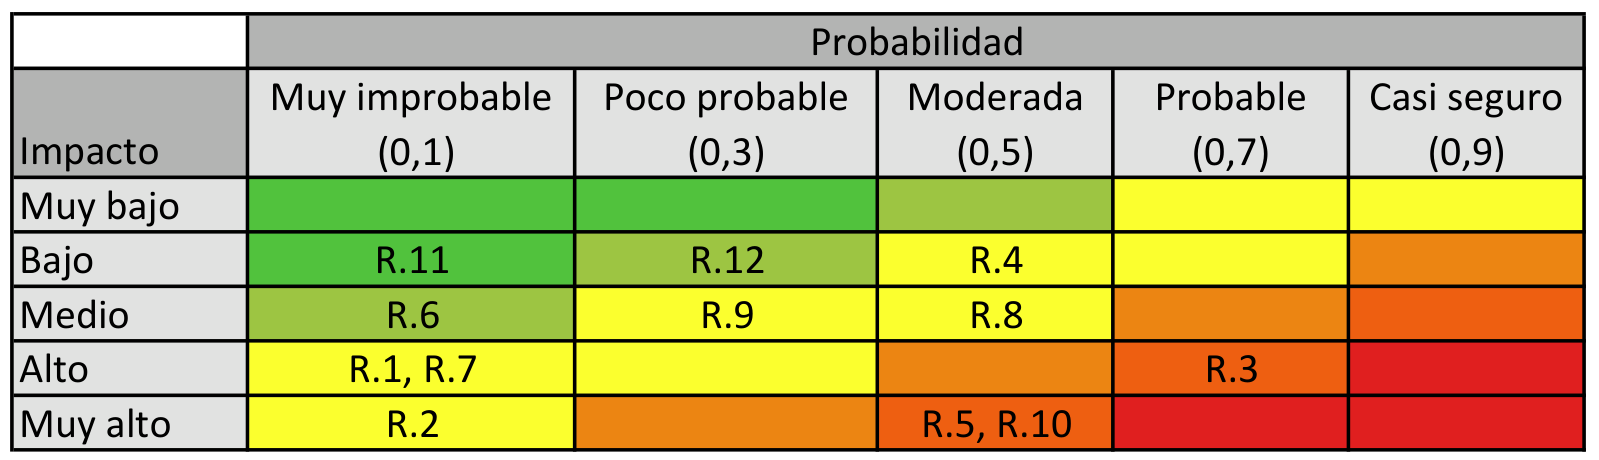
\includegraphics[scale=0.95]{imagenes/planificacion/matriz_riesgos.png}
    \caption{Matriz de probabilidad-impacto de riesgos}
    \label{tabla:riesgos_matriz_probabilidad}
\end{figure}

\subsection{Riesgos materializados}\label{riesgos_materializados}

\textbf{completar esto al final del trabajo, o conforme se vayan ocurriendo}


Los riesgos materializados han estado relacionados principalmente con aspectos técnicos. Primeramente, el R.5. Tuve problemas para instalar OpenBabel en mi máquina por problemas de versiones, por lo que acabé utilizando Google Colab como entorno virtual e instalar ahí algunas librerías necesarias para las primeras experimentaciones con moléculas. Esto tampoco era muy útil a largo plazo puesto que tenía que poder acceder al código fuente para modificarlo, añadir las funcionalidades y compilarlo manualmente para probar los cambios. Por lo que finalmente con ayuda de las guías, se pudo ejecutar localmente. Instantáneamente después, se materializó el riesgo R.3. La falta de conocimiento ante una librería tan grande ya existente retrasó considerablemente el proceso de modificación del código. 
\textbf{Añadir mas riesgos conforme se vayan materializando}

Finalmente, se consiguieron solventar los riesgos manifestados mediante los planes de actuación descritos en cada uno de ellos.
